\documentclass[10pt]{article}

\usepackage{lipsum}
\usepackage{url}
\usepackage{float}
\usepackage{amsmath}
\usepackage{enumitem}
\usepackage{graphicx}
\usepackage{caption}
\usepackage{subcaption}
\usepackage{rotating}
\usepackage{geometry}
\usepackage{listings}
\usepackage{hyperref}
\usepackage[T1]{fontenc}
\usepackage[numbered]{matlab-prettifier}

\newcommand{\documentTitle}{Lab 7 - Digital Logic}
\newcommand{\documentAuthor}{Andrew Pham, Aneel Damaraju}
\newcommand{\courseTitle}{ELEC 240}
\newcommand{\testDate}{October 23, 2018}
\newcommand{\reportDate}{November 2, 2018}

\geometry{margin=1in}
\lstset{
    tabsize=4,
    basicstyle={\ttfamily},
    captionpos=b,
    belowskip=1em,
    aboveskip=1em,
    numbers=left,
	escapechar=\@,
}

\title{
    \textbf{\courseTitle} \\
    \textbf{\documentTitle} \\
    \bigskip
    \textbf{\large{Test performed: \testDate}} \\
    \textbf{\large{Report submitted: \reportDate}} \\
    \bigskip
    \bigskip
}
\author{\documentAuthor}
\date{}

\begin{document}

\maketitle

\newpage

\section{Objective}

The objective of this lab was to learn the underlying logical operations behind an adder and to then apply these principles to implement a one-bit full adder on a breadboard. 

\medskip

%\textit{Note (To be deleted): Think of this test report as a document with your peers as your readers. This means you can assume a similar knowledge background as you. Your readers should be able to easily understand what is going on, and also be able to repeat your lab results based on your document and all references you cite.}

%\textit{For the Objective section, identify the test you performed and its objectives. The objectives of the test are important to state because they are usually analyzed in the conclusion to determine whether the test succeeded.}

\section{Materials}

\begin{itemize}
	\item Test Board
	\item 1x 74HC00 Quad 2-input NAND gate
	\item 1x 7486 Quad 2-input XOR gate
	\item 2x LEDs
	\item 1x Quad DIP switch
	\item 5x 330$\Omega$ resistors
	\item Yellow, Red, and Black wire (signal, power, gnd)
	\item Wire strippers and cutters
\end{itemize}

\medskip

%\textit{Note (To be deleted): Provide a bullet point list of components, software tools, and hardware (such as the NI VirtualBench or DMM) used during the lab}

\section{Test Description}

In the first section of the lab, we learned about the logic underlying the fundamental NAND and XOR gates and their truth tables for all combinations of inputs. We then formulated an expression for the correct output of the adder for the three input bits. We then applied DeMorgan's law to simplify the circuit so that it only uses NAND and XOR gates, and we then constructed the one-bit full adder. 

\medskip

%\textit{Note (To be deleted): This section provides a summary of the test your team performed. Give enough information so readers can understand what you did, but do not go into the details of every step.}

\subsection{Pre-Lab Calculations and Schematics}
To begin, we had to understand the underlying logic behind a NAND and a XOR gate, which the adder was composed of. Below in Figure \ref{NAND} is the truth table for a NAND gate, and in Figure \ref{XOR} is the truth table for a XOR gate. 

\begin{figure} [H]
	\begin{table}[H]
		\centering
		\begin{tabular}{||c c c||} 
			\hline
			A & B &  A NAND B\\ [0.5ex] 
			\hline\hline
			0 & 0 & 1\\ 
			0 & 1 & 1\\
			1 & 0 & 1\\
			1 & 1 & 0\\ [1ex] 
			\hline
		\end{tabular}
	\end{table}
	\caption{NAND Truth Table}
	\label{NAND}
\end{figure}

\begin{figure} [H]
	\begin{table}[H]
		\centering
		\begin{tabular}{||c c c||} 
			\hline
			A & B &  A NAND B\\ [0.5ex] 
			\hline\hline
			0 & 0 & 0\\ 
			0 & 1 & 1\\
			1 & 0 & 1\\
			1 & 1 & 0\\ [1ex] 
			\hline
		\end{tabular}
	\end{table}
	\caption{XOR Truth Table}
	\label{XOR}
\end{figure}

We then derived the following expression for the Sum $S$ and Carry $C$ output bits of the adder based on the three one-bit inputs $x,y,z$. 

$$ S = (x \bigoplus y) \bigoplus z$$
$$ C = (x \bullet y) \vee (x \bigoplus y) \bullet z $$

We then created the following truth table for the sum and carry bits based on these outputs as follows in Fig \ref{sum}:

\begin{figure} [H]
	\begin{table}[H]
		\centering
		\begin{tabular}{||c c c c c c c c c||} 
			\hline
			x & y &  z & $x \bullet y$ & $x \bigoplus y$ & $(x \bigoplus y) \bigoplus z$ & $ (x \bullet y) \vee (x \bigoplus y) $ & C & S\\ [0.5ex] 
			\hline\hline
			0 & 0 & 0 & 0 & 0 & 0 & 0 & 0 & 0\\ 
			0 & 0 & 1 & 0 & 0 & 1 & 0 & 0 & 1\\
			0 & 1 & 0 & 0 & 1 & 1 & 1 & 0 & 1\\
			0 & 1 & 1 & 0 & 1 & 0 & 1 & 1 & 0\\
			1 & 0 & 0 & 0 & 1 & 1 & 1 & 0 & 1\\
			1 & 0 & 1 & 0 & 1 & 0 & 1 & 1 & 0\\
			1 & 1 & 0 & 0 & 0 & 1 & 0 & 0 & 1\\
			1 & 1 & 1 & 1 & 0 & 1 & 1 & 1 & 1\\[1ex] 
			\hline
		\end{tabular}
	\end{table}
	\caption{Naive Truth Table for the Sum and Carry bits}
	\label{sum}
\end{figure}

However, the direct implementation of the above truth table into logic requires the use of 2 XOR gates for the sum bit 2 NAND gates, and 1 OR gate for the carry bit. Since we want to reduce the complexity of our adder, we can use DeMorgan's laws to simplify the requirements for the carry bits:

$$ x \bullet y = \lnot (x \vee y) $$
$$ x \vee y = \lnot (x \bullet y) $$

We then obtain the following equation for the carry bit expression by applying the above DeMorgan's laws:

$$ C = \lnot 
\left( 
\lnot (x \bullet y) \bullet \lnot 
\left( 
\left(x \bigoplus y \right) \bullet z 
\right) 
\right) $$

The truth table is depicted below in Fig \ref{mod};

\begin{figure} [H]
	\begin{table}[H]
		\centering
		\begin{tabular}{||c c c c c c c c||} 
			\hline
			x & y &  z & $x \bullet y$ & $x \bigoplus y$ & $\lnot ((x \bigoplus y) \bullet z)$ & $ \lnot(x \bullet y) \bullet \lnot ((x \bigoplus y) \bullet z)$ & C\\ [0.5ex] 
			\hline\hline
			0 & 0 & 0 & 0 & 0 & 1 & 1 & 0\\ 
			0 & 0 & 1 & 0 & 0 & 1 & 1 & 0\\
			0 & 1 & 0 & 0 & 1 & 1 & 1 & 0\\
			0 & 1 & 1 & 0 & 1 & 0 & 0 & 1\\
			1 & 0 & 0 & 0 & 1 & 1 & 1 & 0\\
			1 & 0 & 1 & 0 & 1 & 0 & 0 & 1\\
			1 & 1 & 0 & 0 & 0 & 1 & 1 & 0\\
			1 & 1 & 1 & 1 & 0 & 1 & 0 & 1\\[1ex] 
			\hline
		\end{tabular}
	\end{table}
	\caption{Modified Truth Table for the Sum and Carry bits}
	\label{mod}
\end{figure}

The circuit that implements this truth table's equation is depicted below in Fig \ref{fig:circuit} :

\begin{centering}
	\begin{figure} [H]
		\centering
		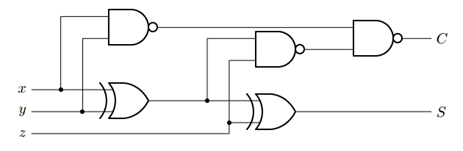
\includegraphics[scale=0.75]{images/fulladder_2.png}
		\caption{One-Bit Full Adder Circuit Diagram}
		\label{fig:circuit}
	\end{figure}
\end{centering}

\medskip

%\textit{Note (To be deleted): Include the homework pre-calculations and schematics that serve as the initial setup for the test. Briefly explain the importance of each item you include. You may want to number your equations/figures so you can refer to them in later sections. Including photos of handwritten work is okay.}

\section{Results and Discussion}

\subsection{Part A: Understanding the components}

Before understanding an adder, it is important to learn what the components are and what they do. The list of components used in the circuit are mentioned in the materials, with the relevant logic materials being the LED, Quad DIP switch and XOR and NAND gate. The LED is useful as a display, as having two LED's effectively displays all possible two bit combinations from 00 to 11 in binary or 0 to 3 in decimal. The Quad DIP switch is used to convey which bits will be added, up to a maximum of three. The XOR and NAND gates perform their desired intended logical function on the two input bits, and will be implemented as parts of the adder.

\subsection{Part B: The Full-Adder Circuit}

This section was pretty straight forward, but was an attempt to understand how to implement a full adder in  terms of the circuit components. The truth table for the full-adder can be seen in Figure \ref{sum}. However, this table does not take into account the current physical limitations, of only having NAND and XOR gates. This can be seen in Figure \ref{mod} which has taken into account DeMorgan's law and thus only uses NAND and XOR gates. 

\subsection{Part C: Constructing the Full-Adder}

As the name implies, this section is devoted to using by creating the Full-Adder circuit physically. The steps taken toward creating the logical circuit can be seen in Figure \ref{fig:circuit}. The only steps needed after creating this are attaching the x,y and z bits as well as displaying the carry and sum bit outputs. The inputs are created by attaching 3 of the 4 switches on the quad DIP to power and ground, with each of the switches acting as a different input bit. For the output bits, connecting an led resistor combination through each of the outputs will create a 1 or a 0 bit. The output for each of the bits can be seen below.

\begin{centering}
	\begin{figure} [H]
		\centering
		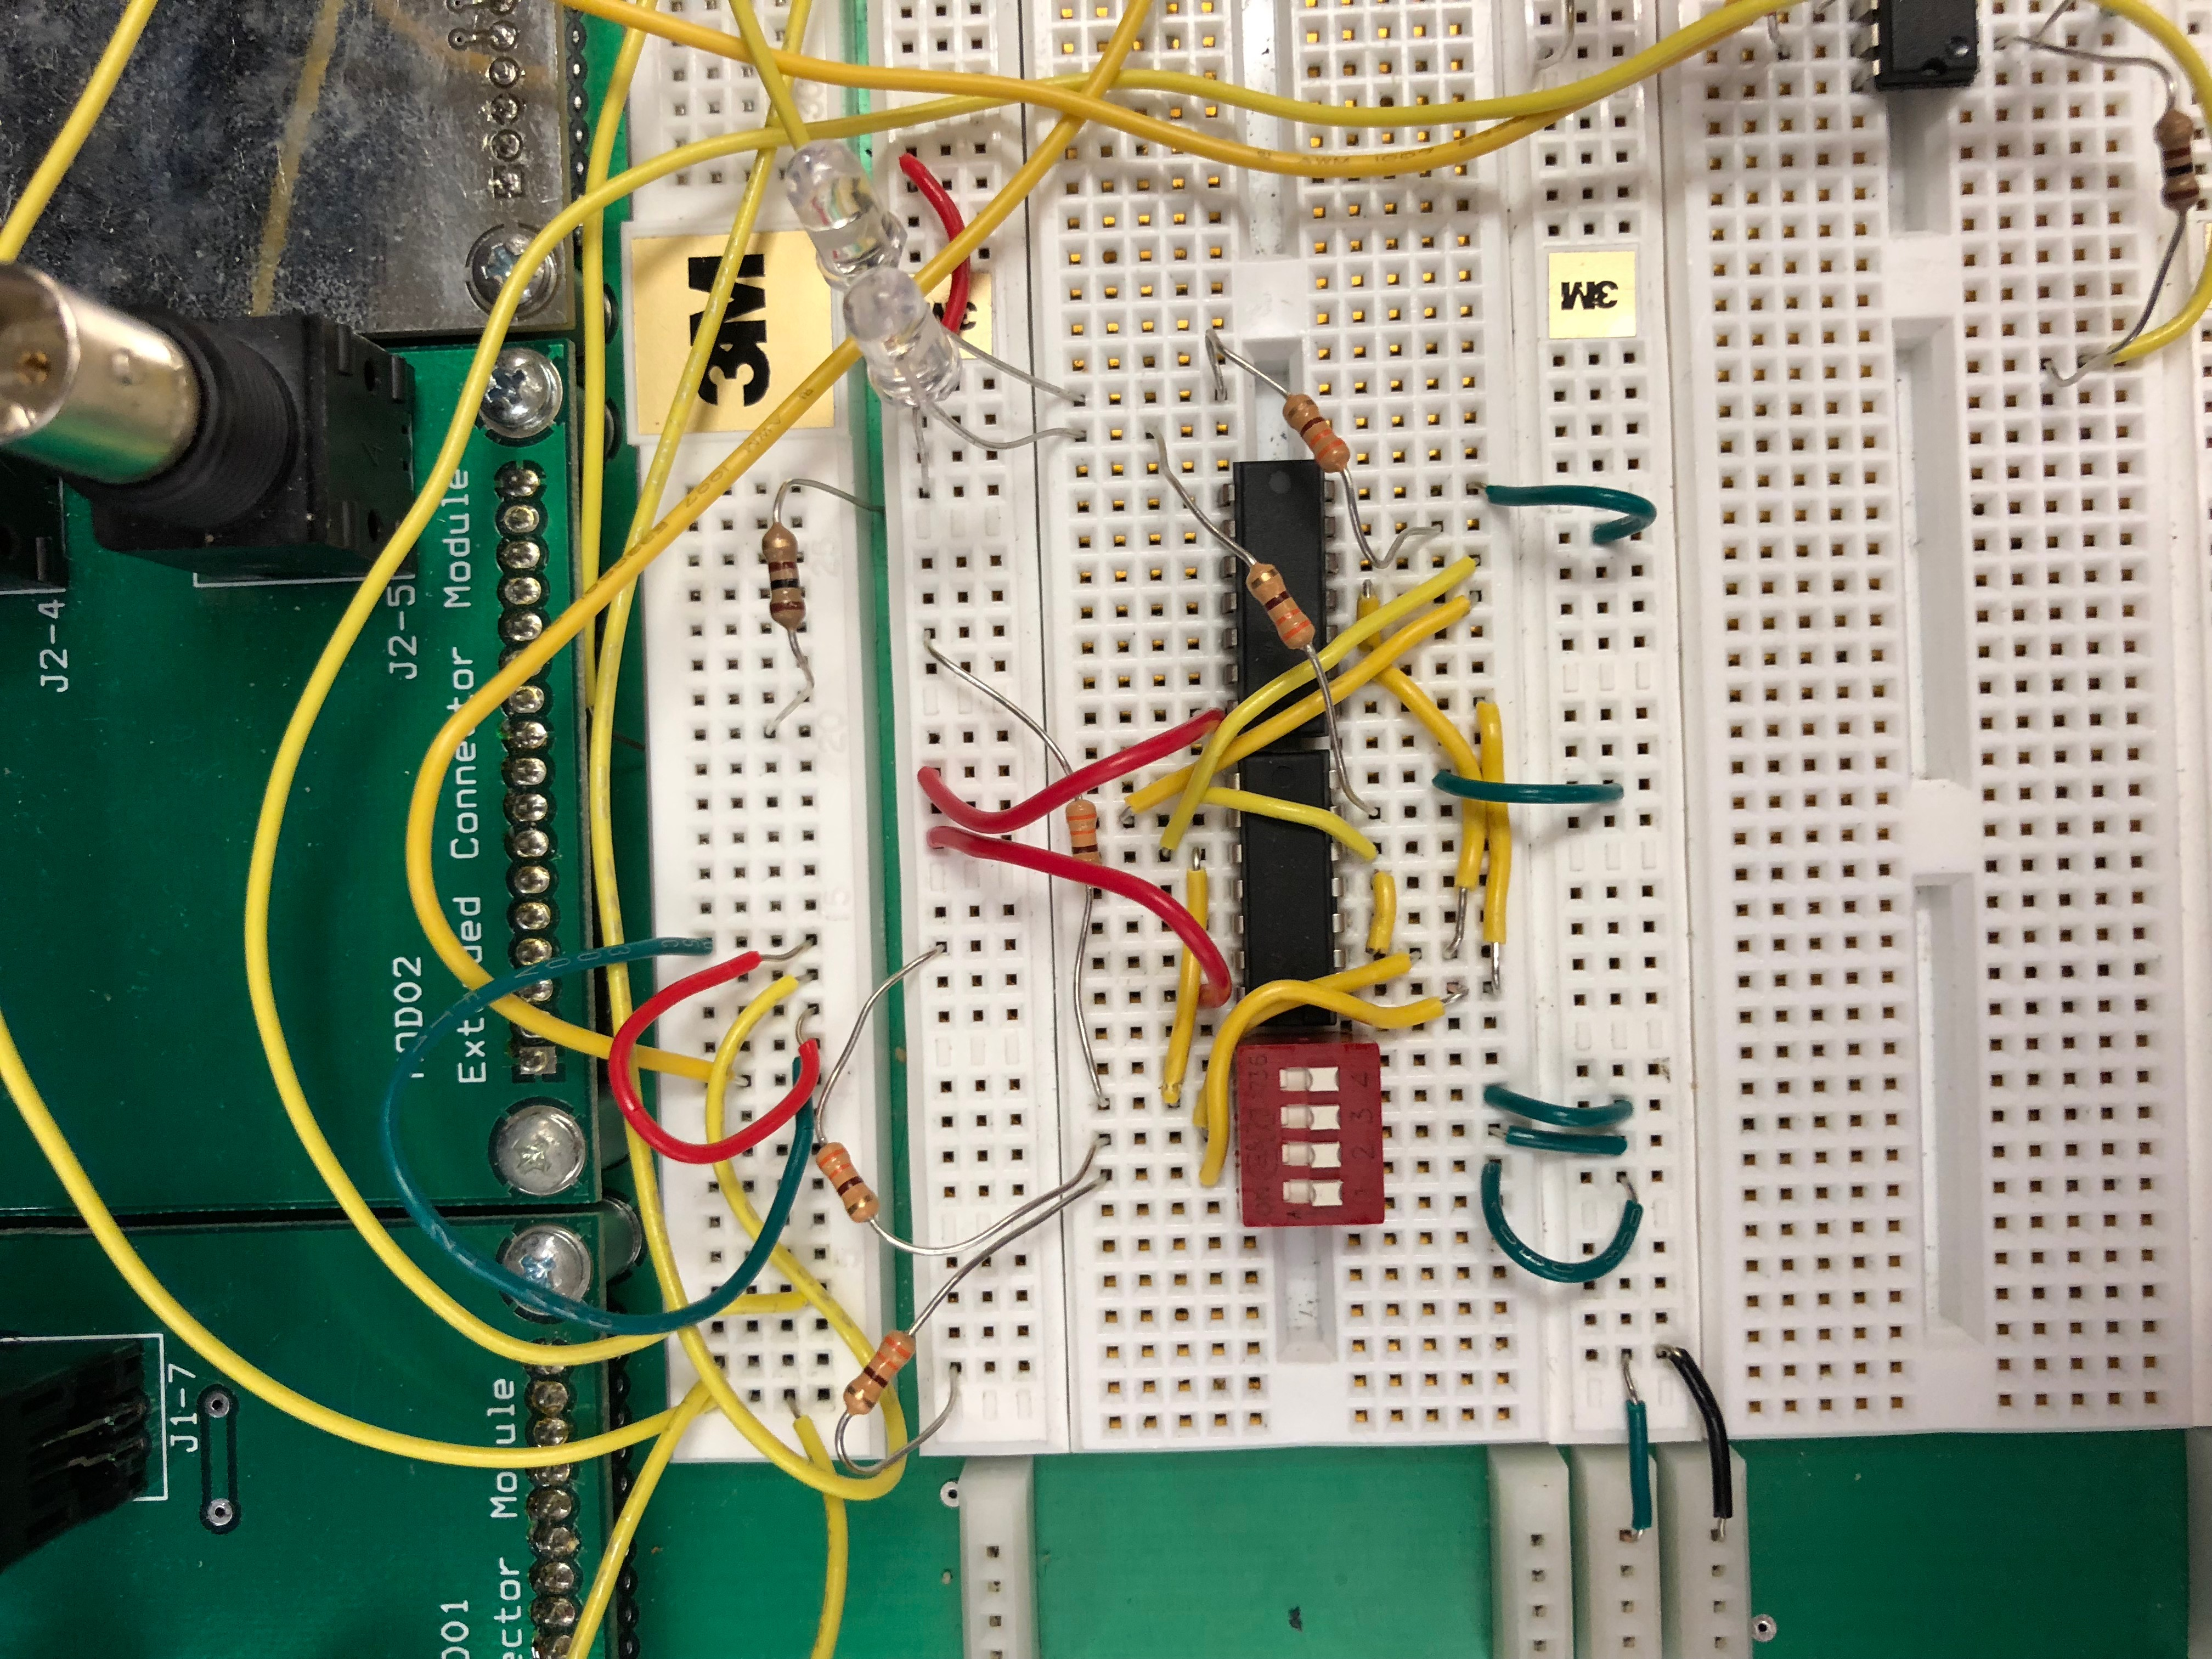
\includegraphics[scale=0.07]{images/000led.jpg}
		\caption{000 Input with 00 Output}
	\end{figure}
\end{centering}

\begin{centering}
	\begin{figure} [H]
		\centering
		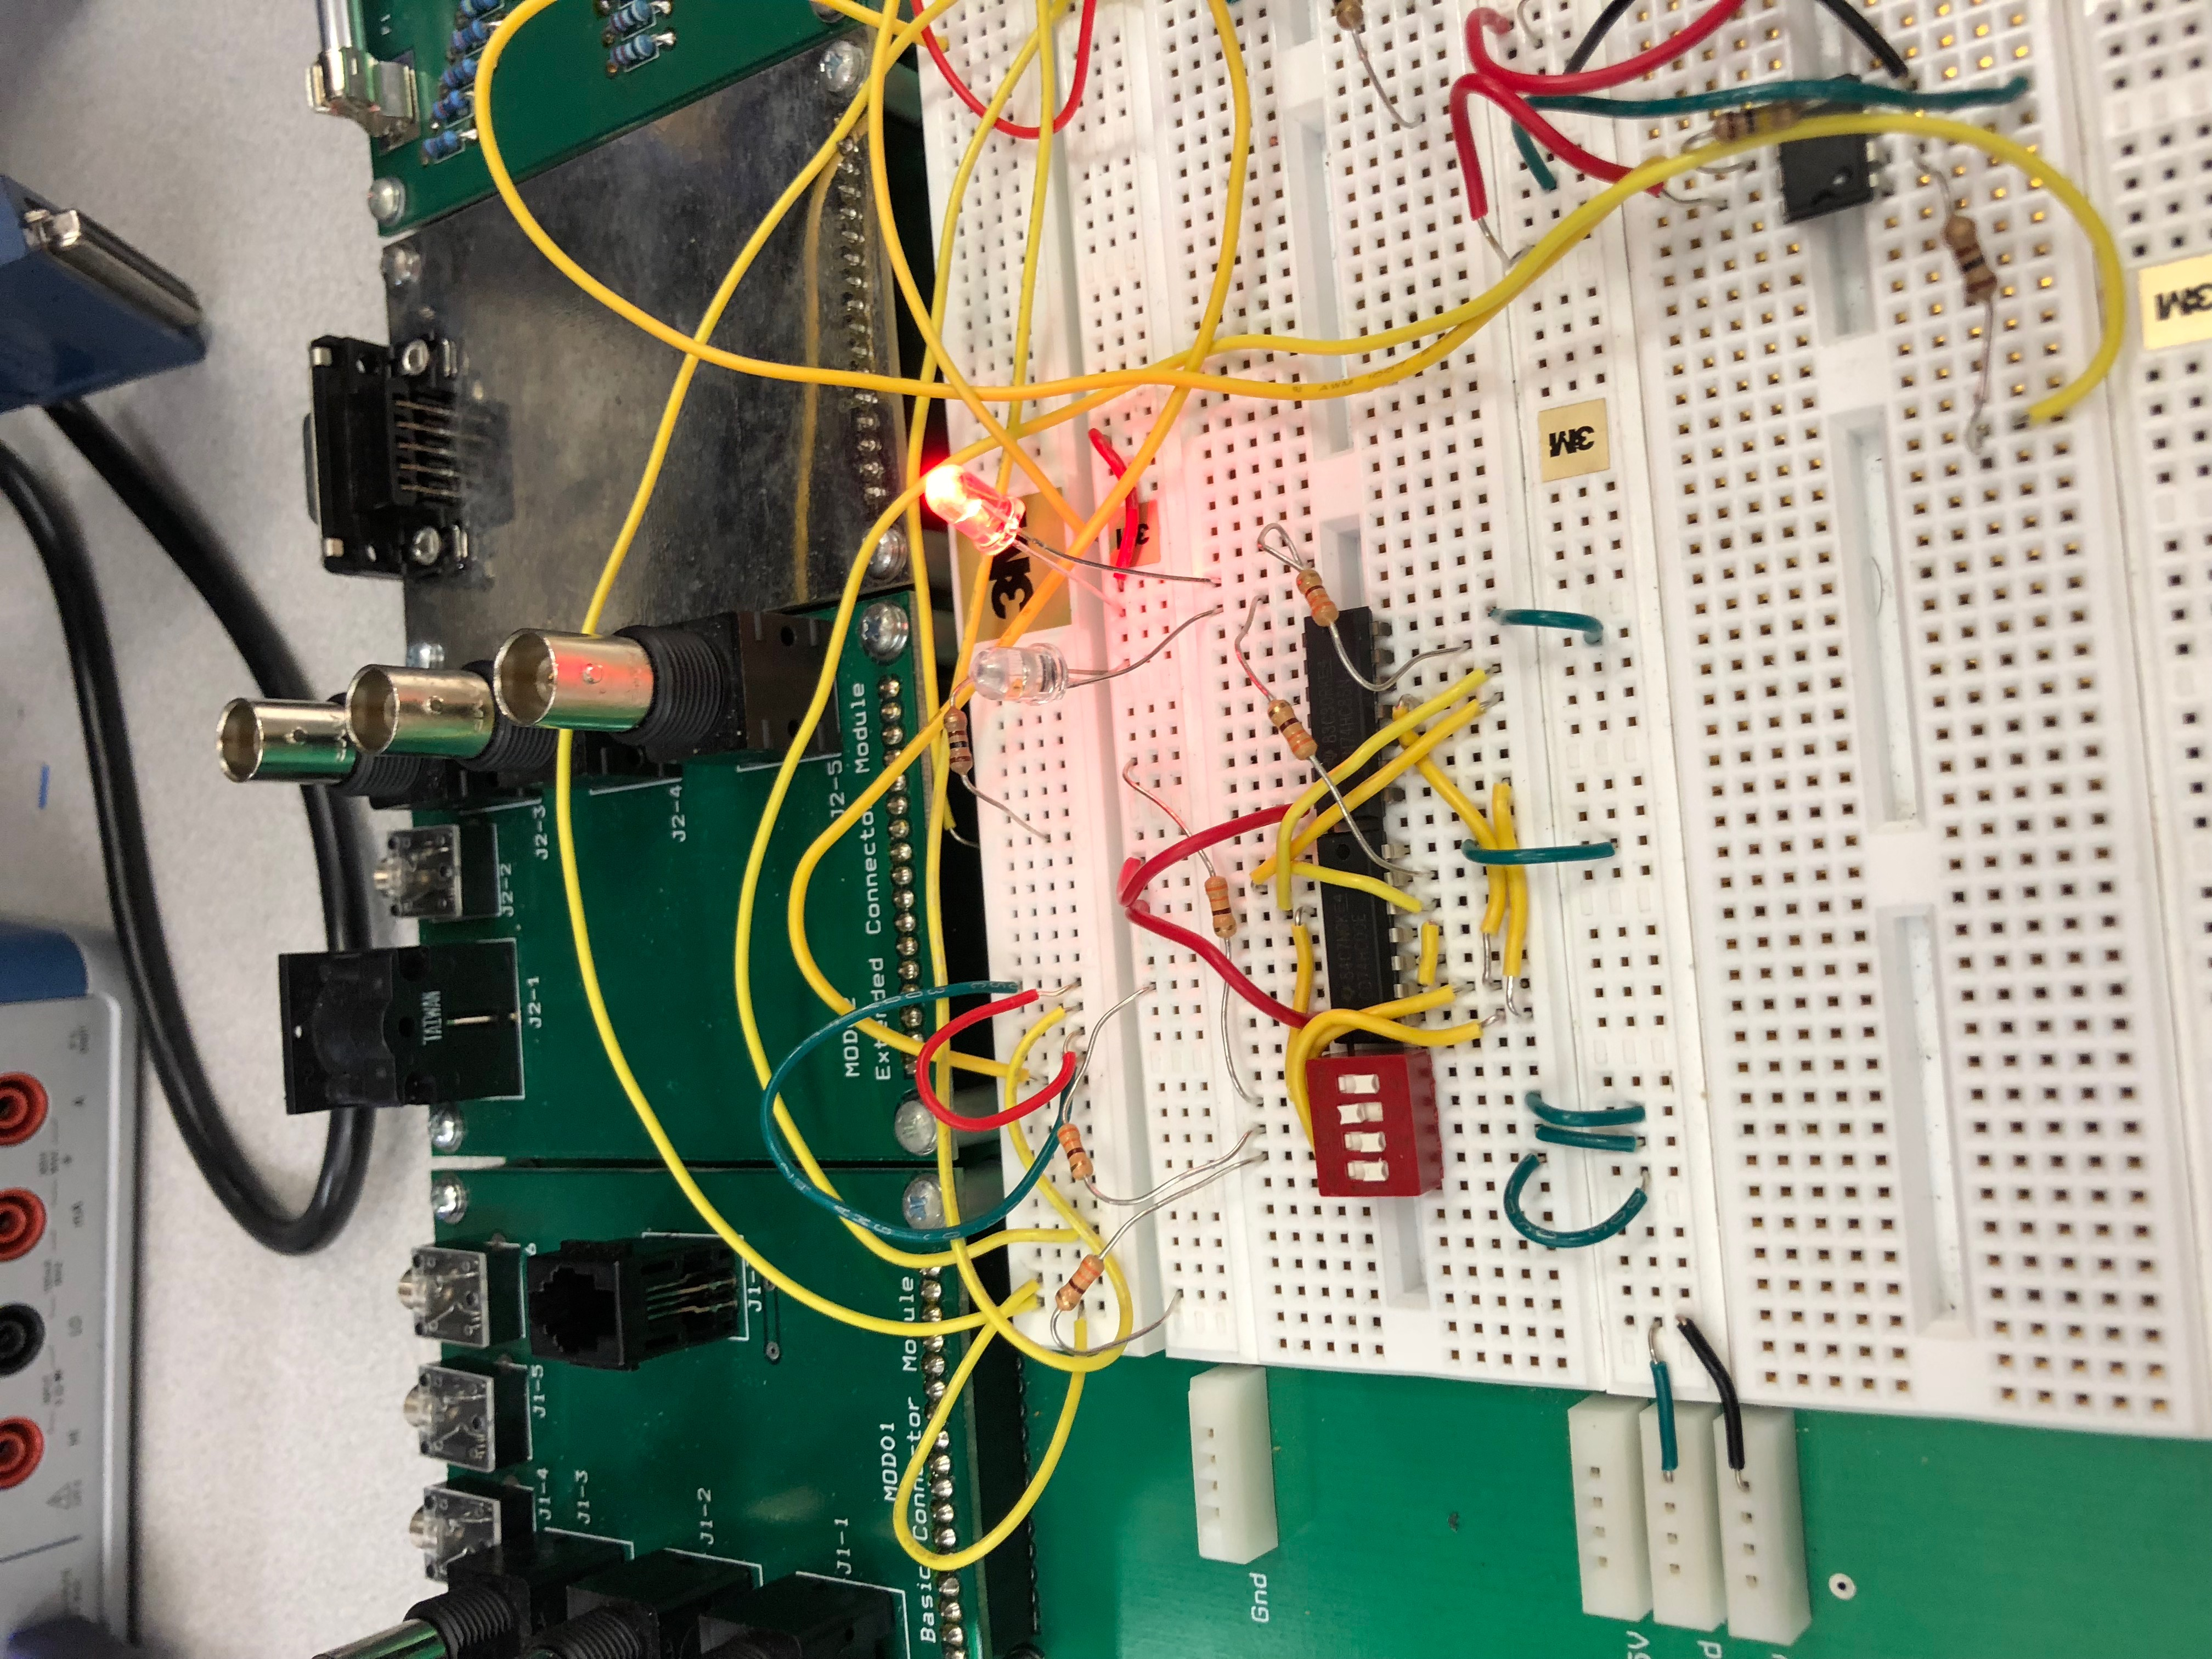
\includegraphics[scale=0.07]{images/001led.jpg}
		\caption{001 Input with 01 Output}
	\end{figure}
\end{centering}

\begin{centering}
	\begin{figure} [H]
		\centering
		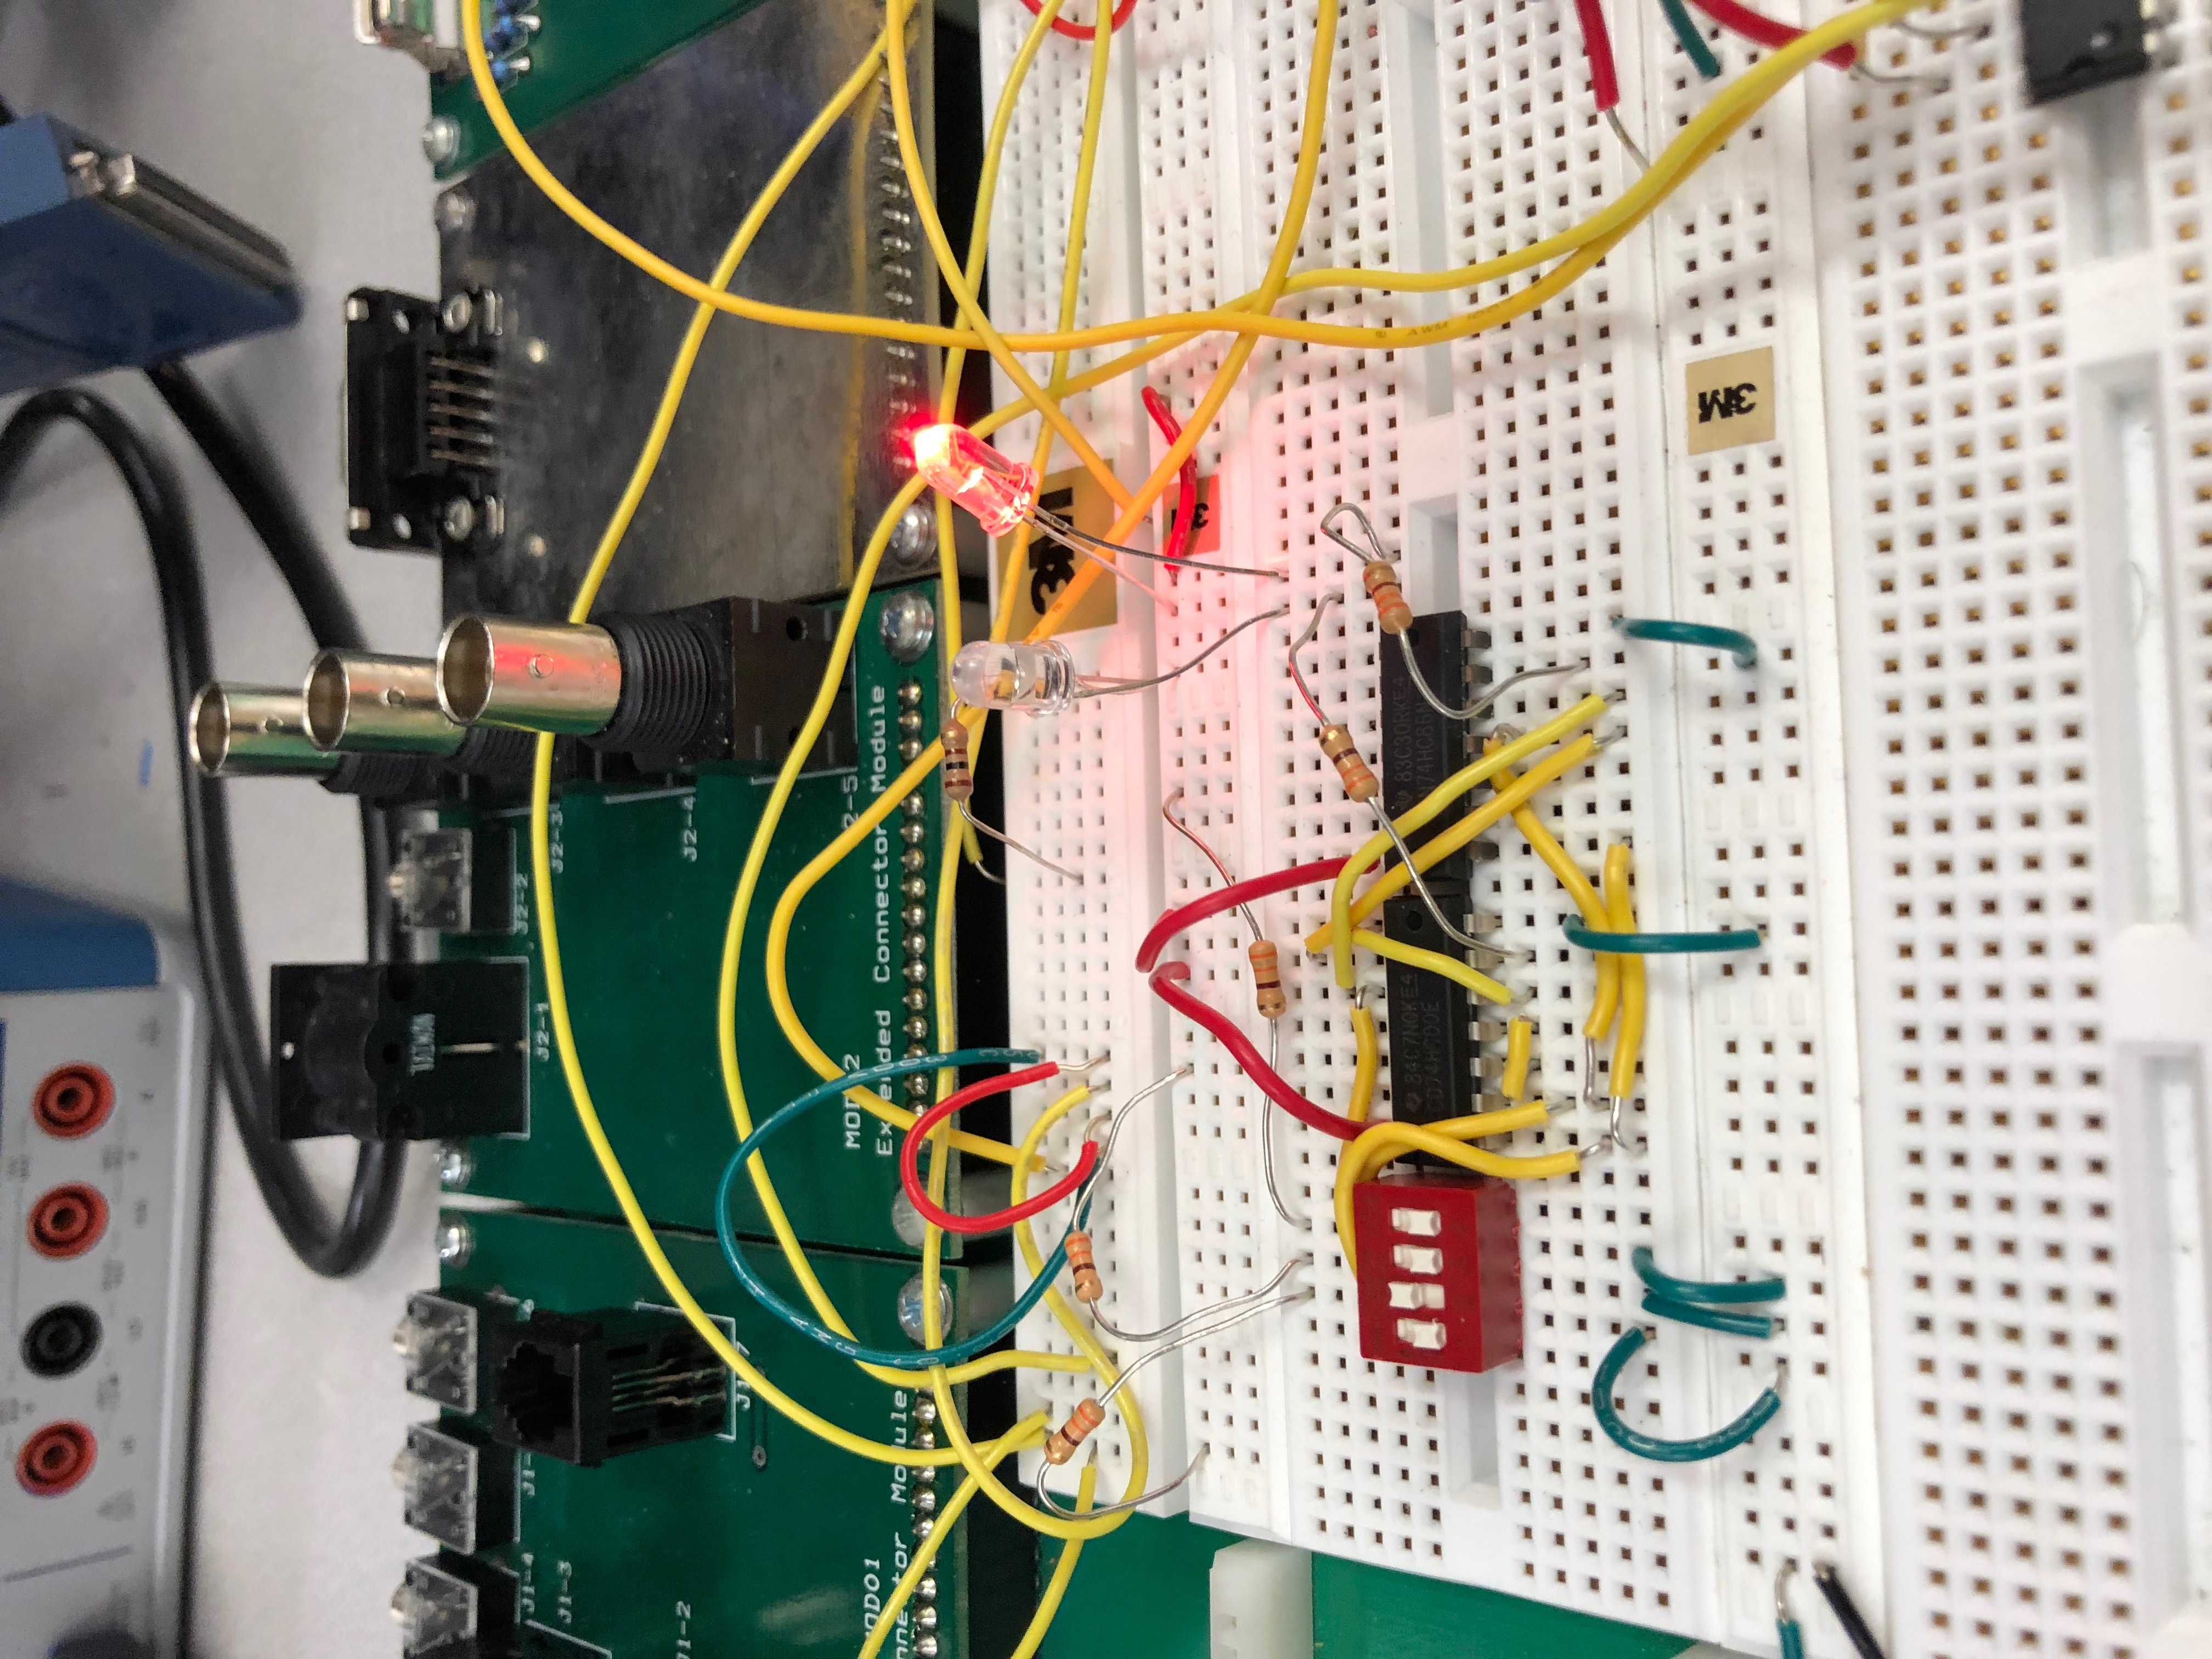
\includegraphics[scale=0.07]{images/010led.jpg}
		\caption{010 Input with 01 Output}
	\end{figure}
\end{centering}

\begin{centering}
	\begin{figure} [H]
		\centering
		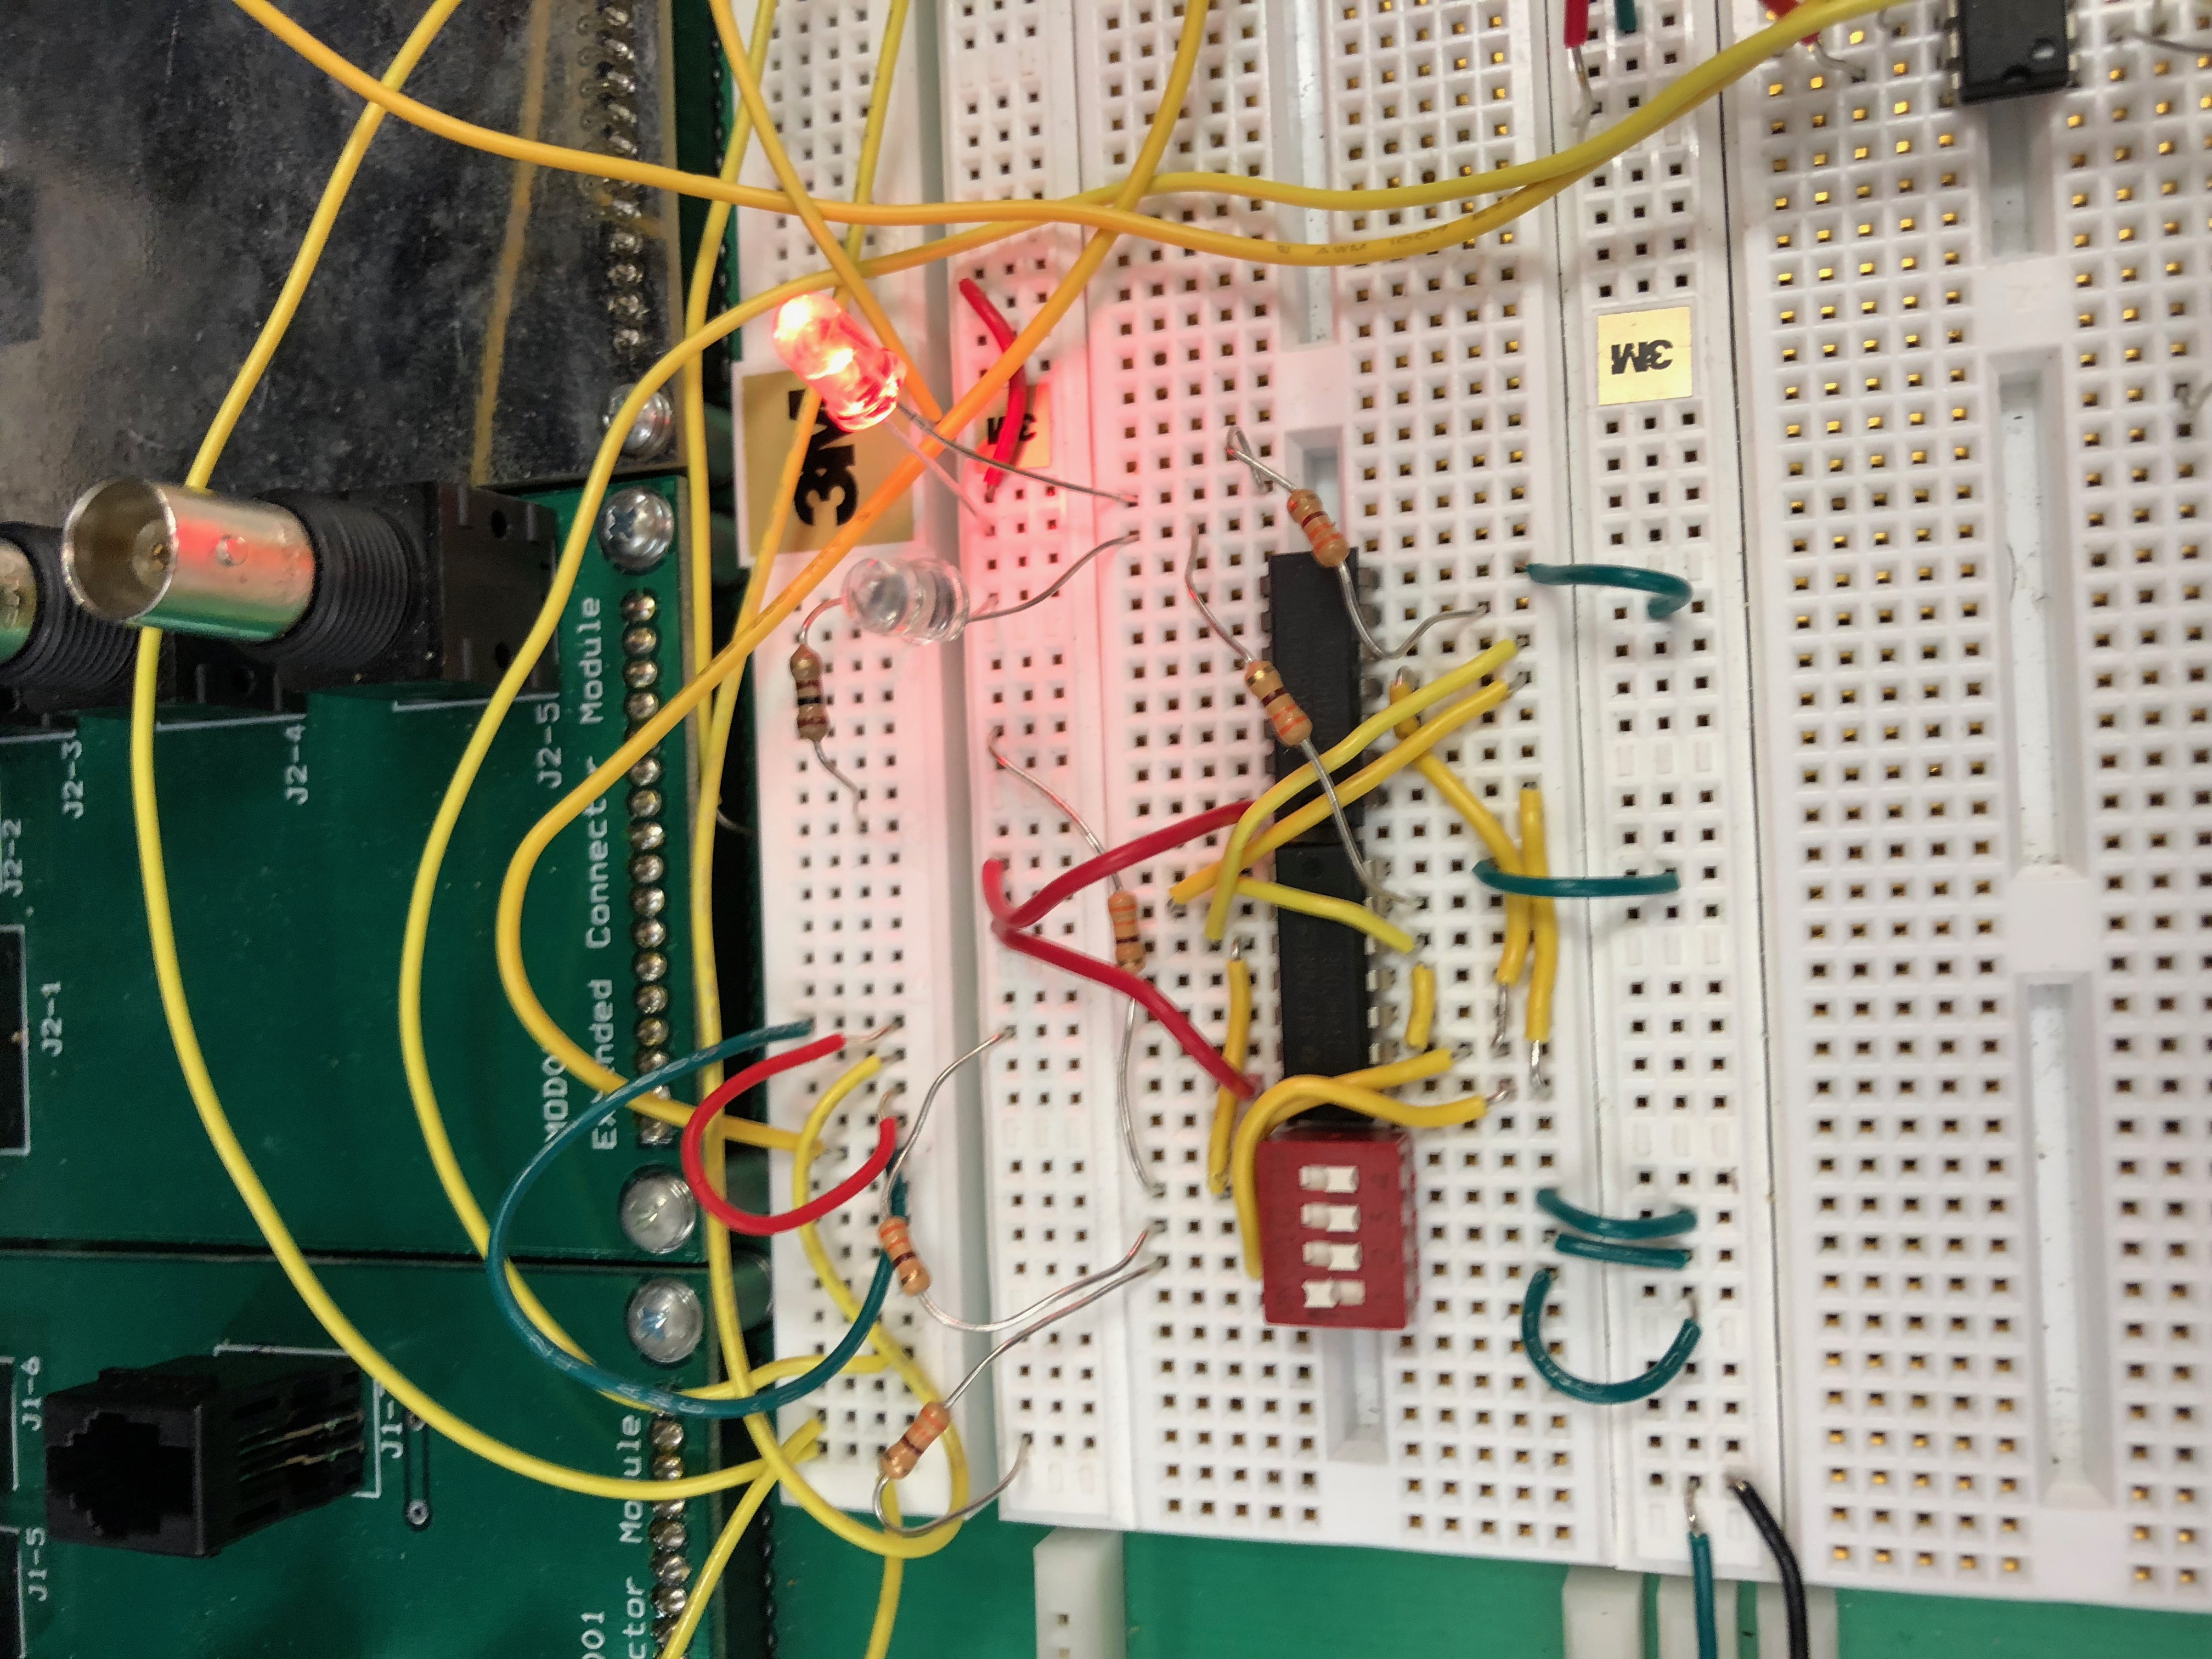
\includegraphics[scale=0.07]{images/100led.jpg}
		\caption{100 Input with 01 Output}
	\end{figure}
\end{centering}

\begin{centering}
	\begin{figure} [H]
		\centering
		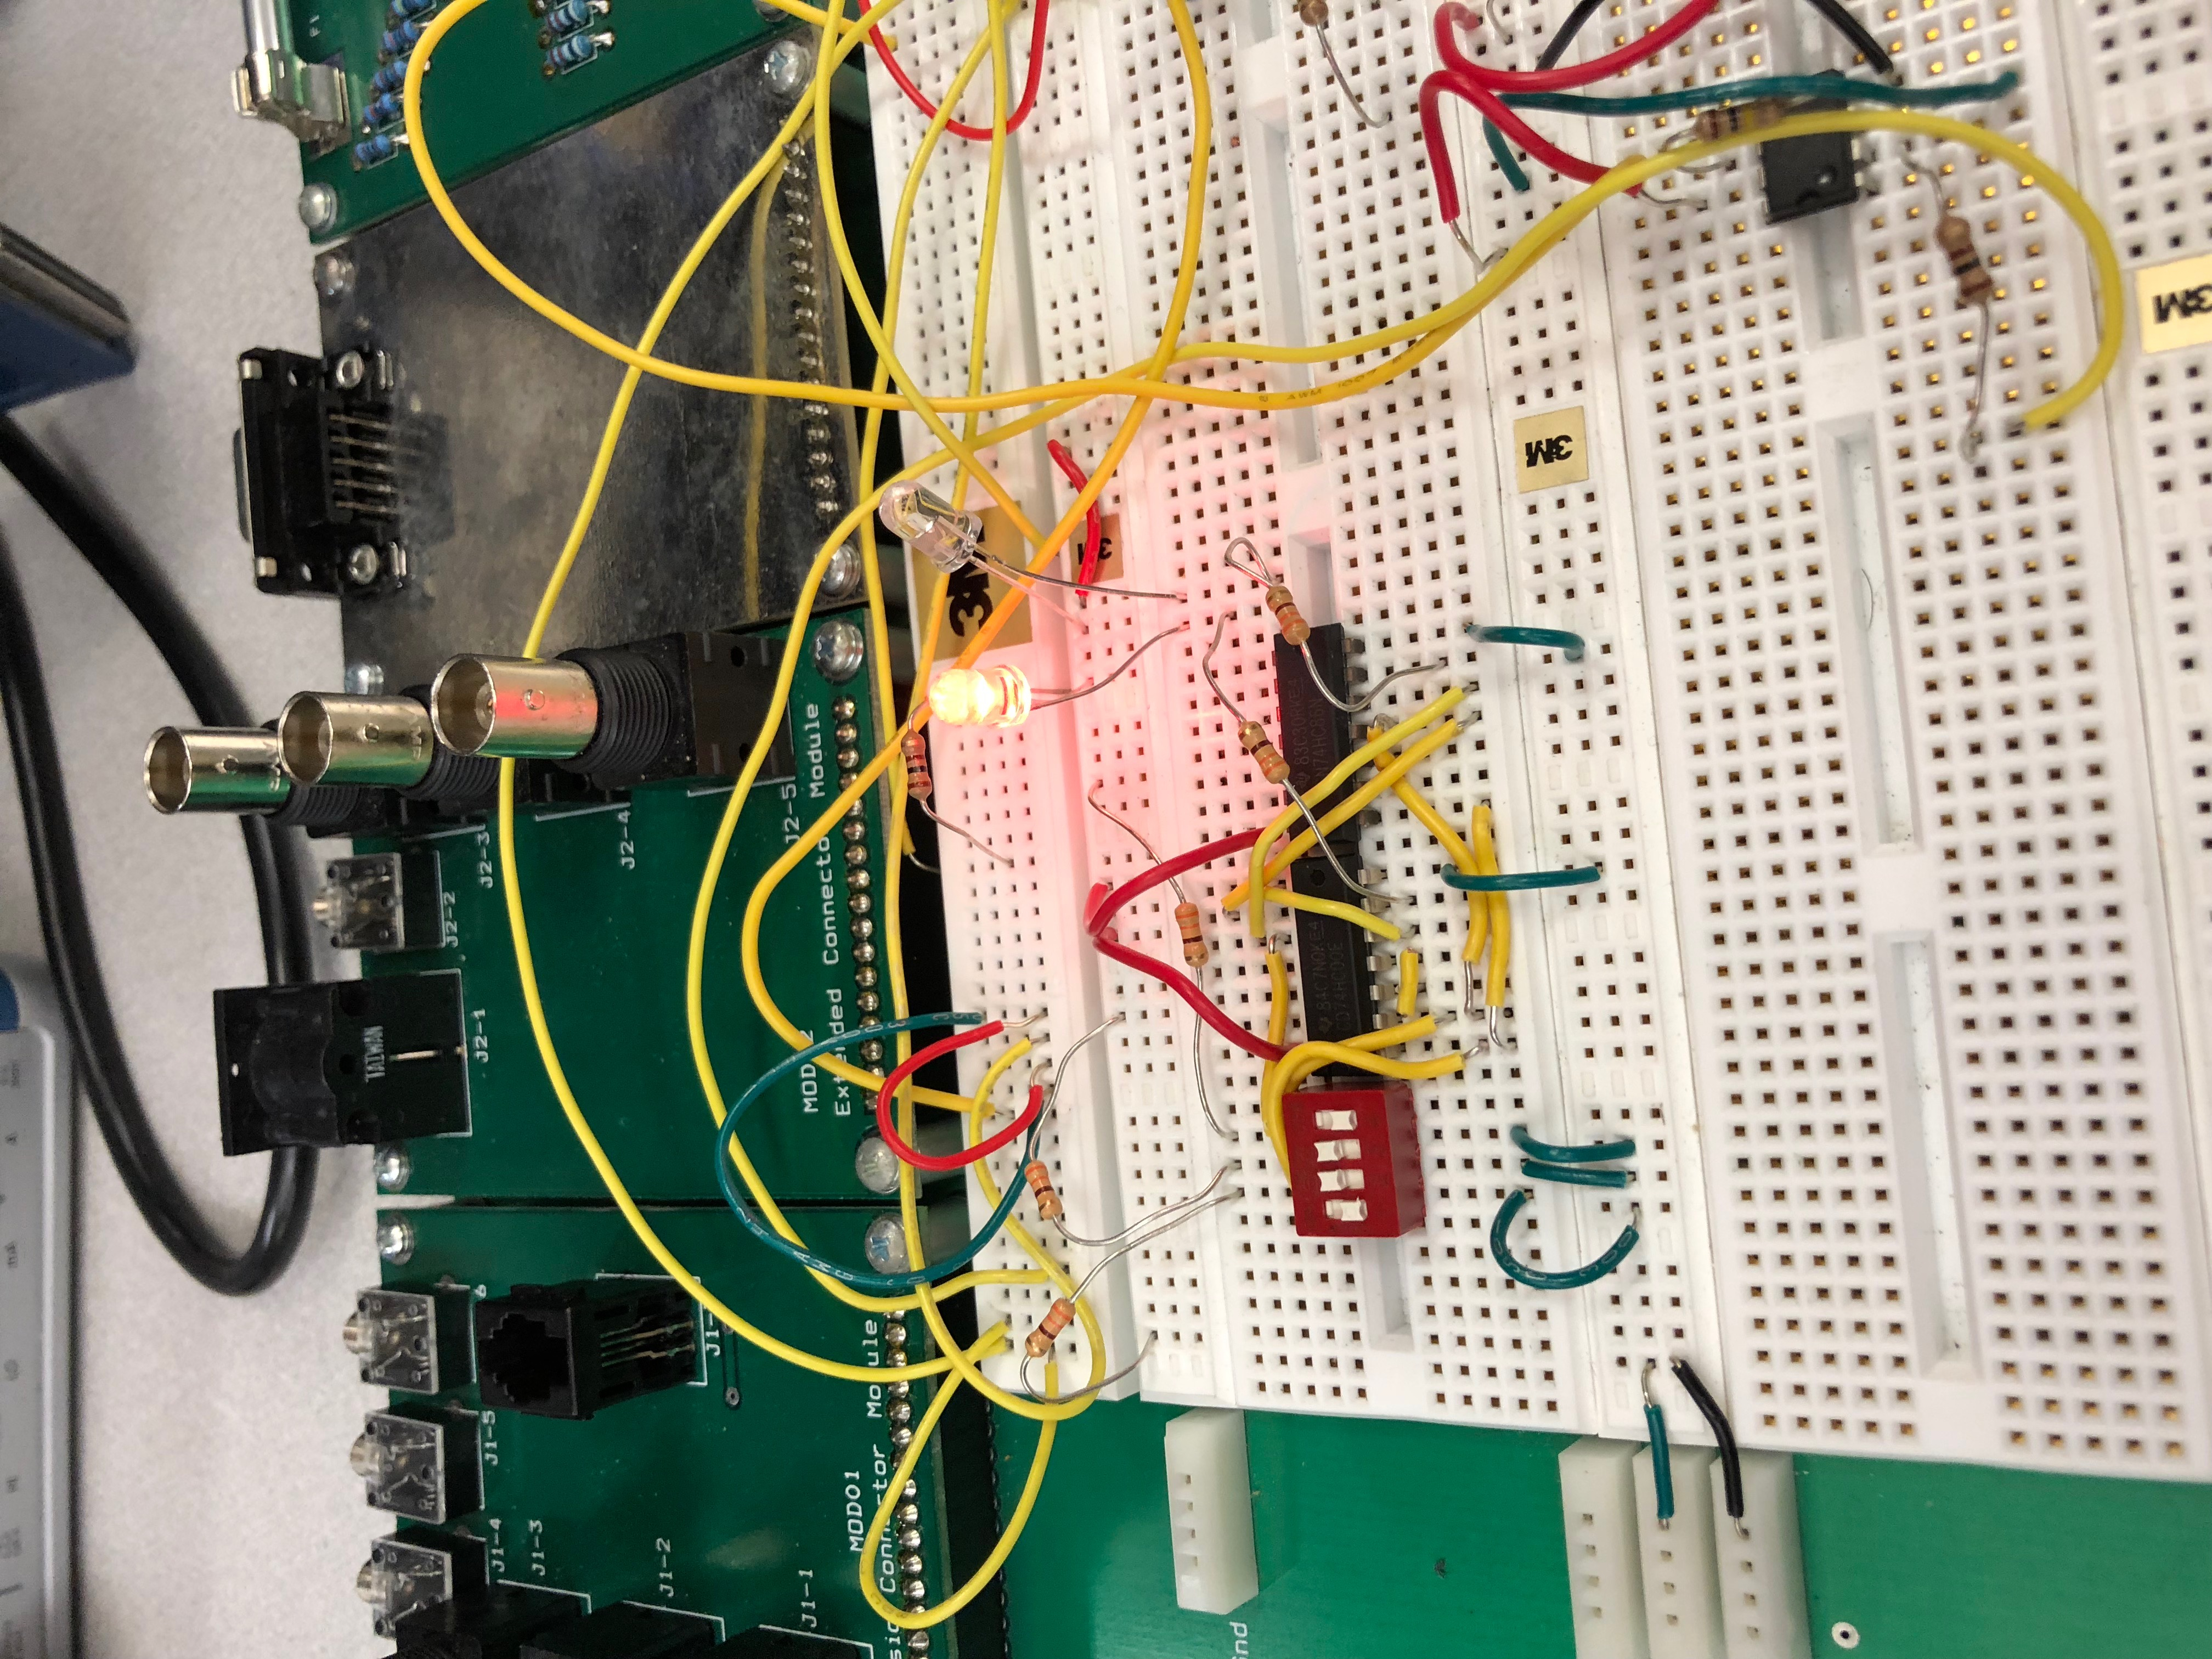
\includegraphics[scale=0.07]{images/011led.jpg}
		\caption{011Input with 10 Output}
	\end{figure}
\end{centering}

\begin{centering}
	\begin{figure} [H]
		\centering
		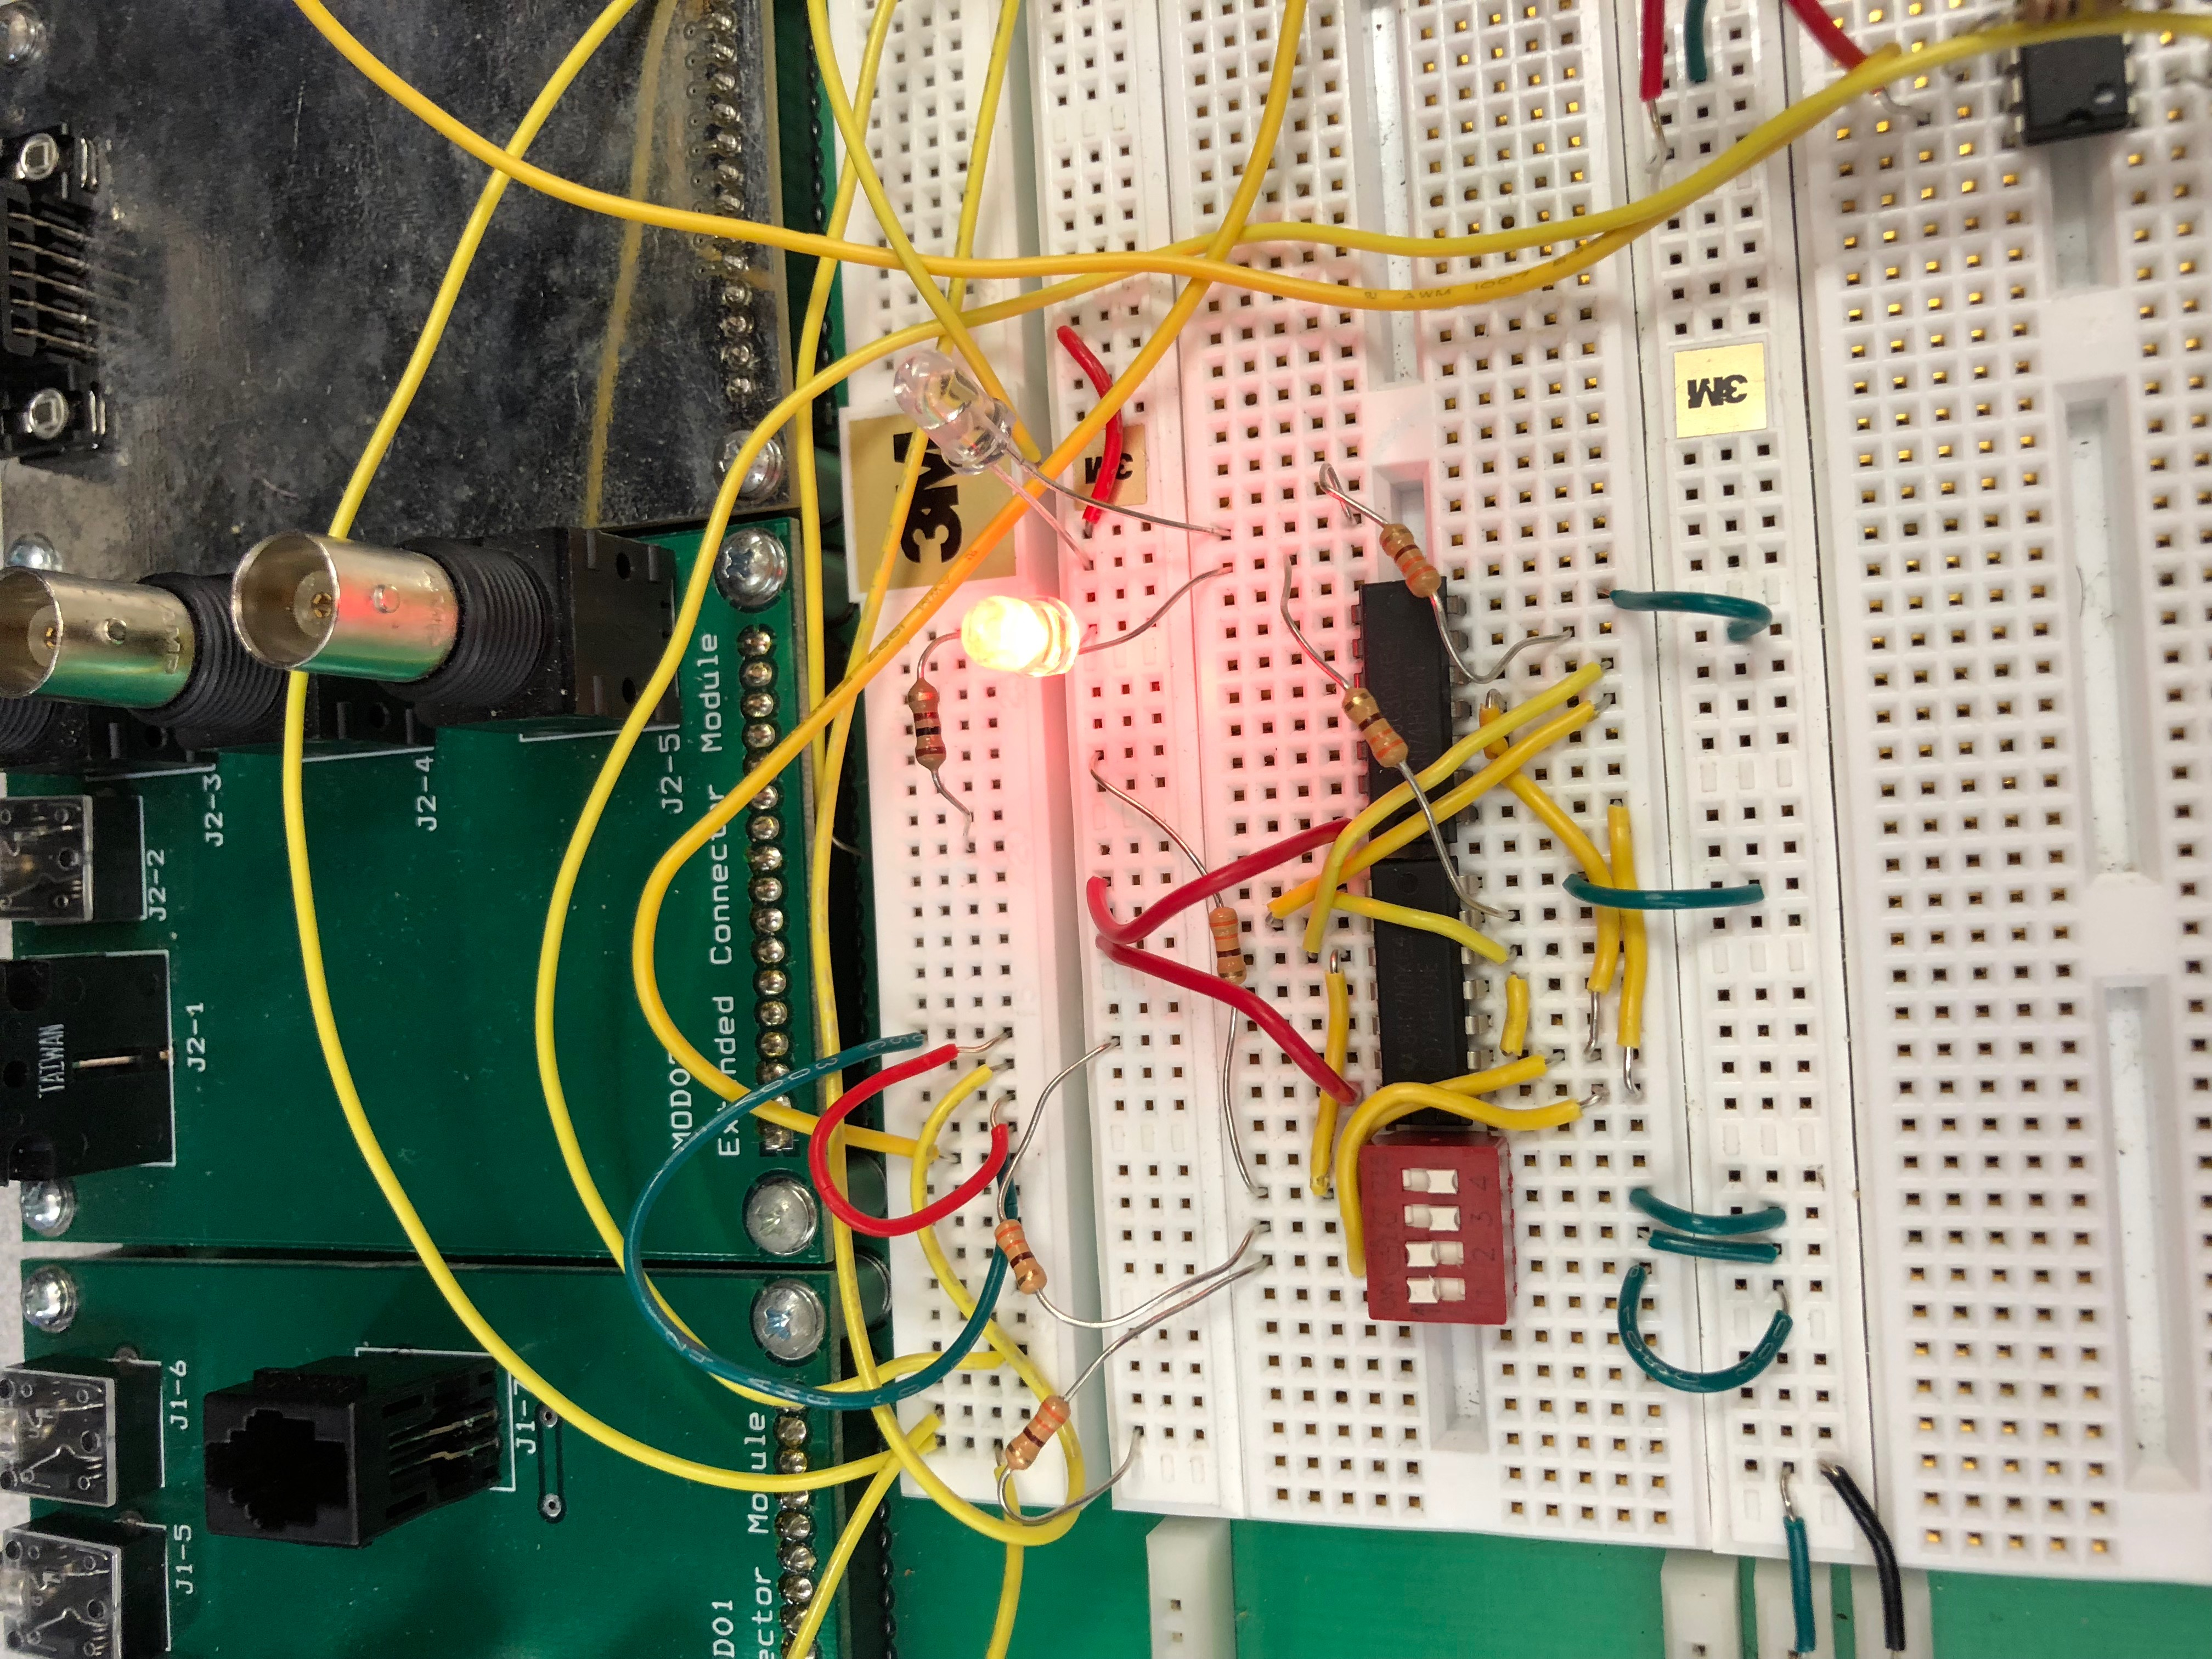
\includegraphics[scale=0.07]{images/110led.jpg}
		\caption{110 Input with 10 Output}
	\end{figure}
\end{centering}

\begin{centering}
	\begin{figure} [H]
		\centering
		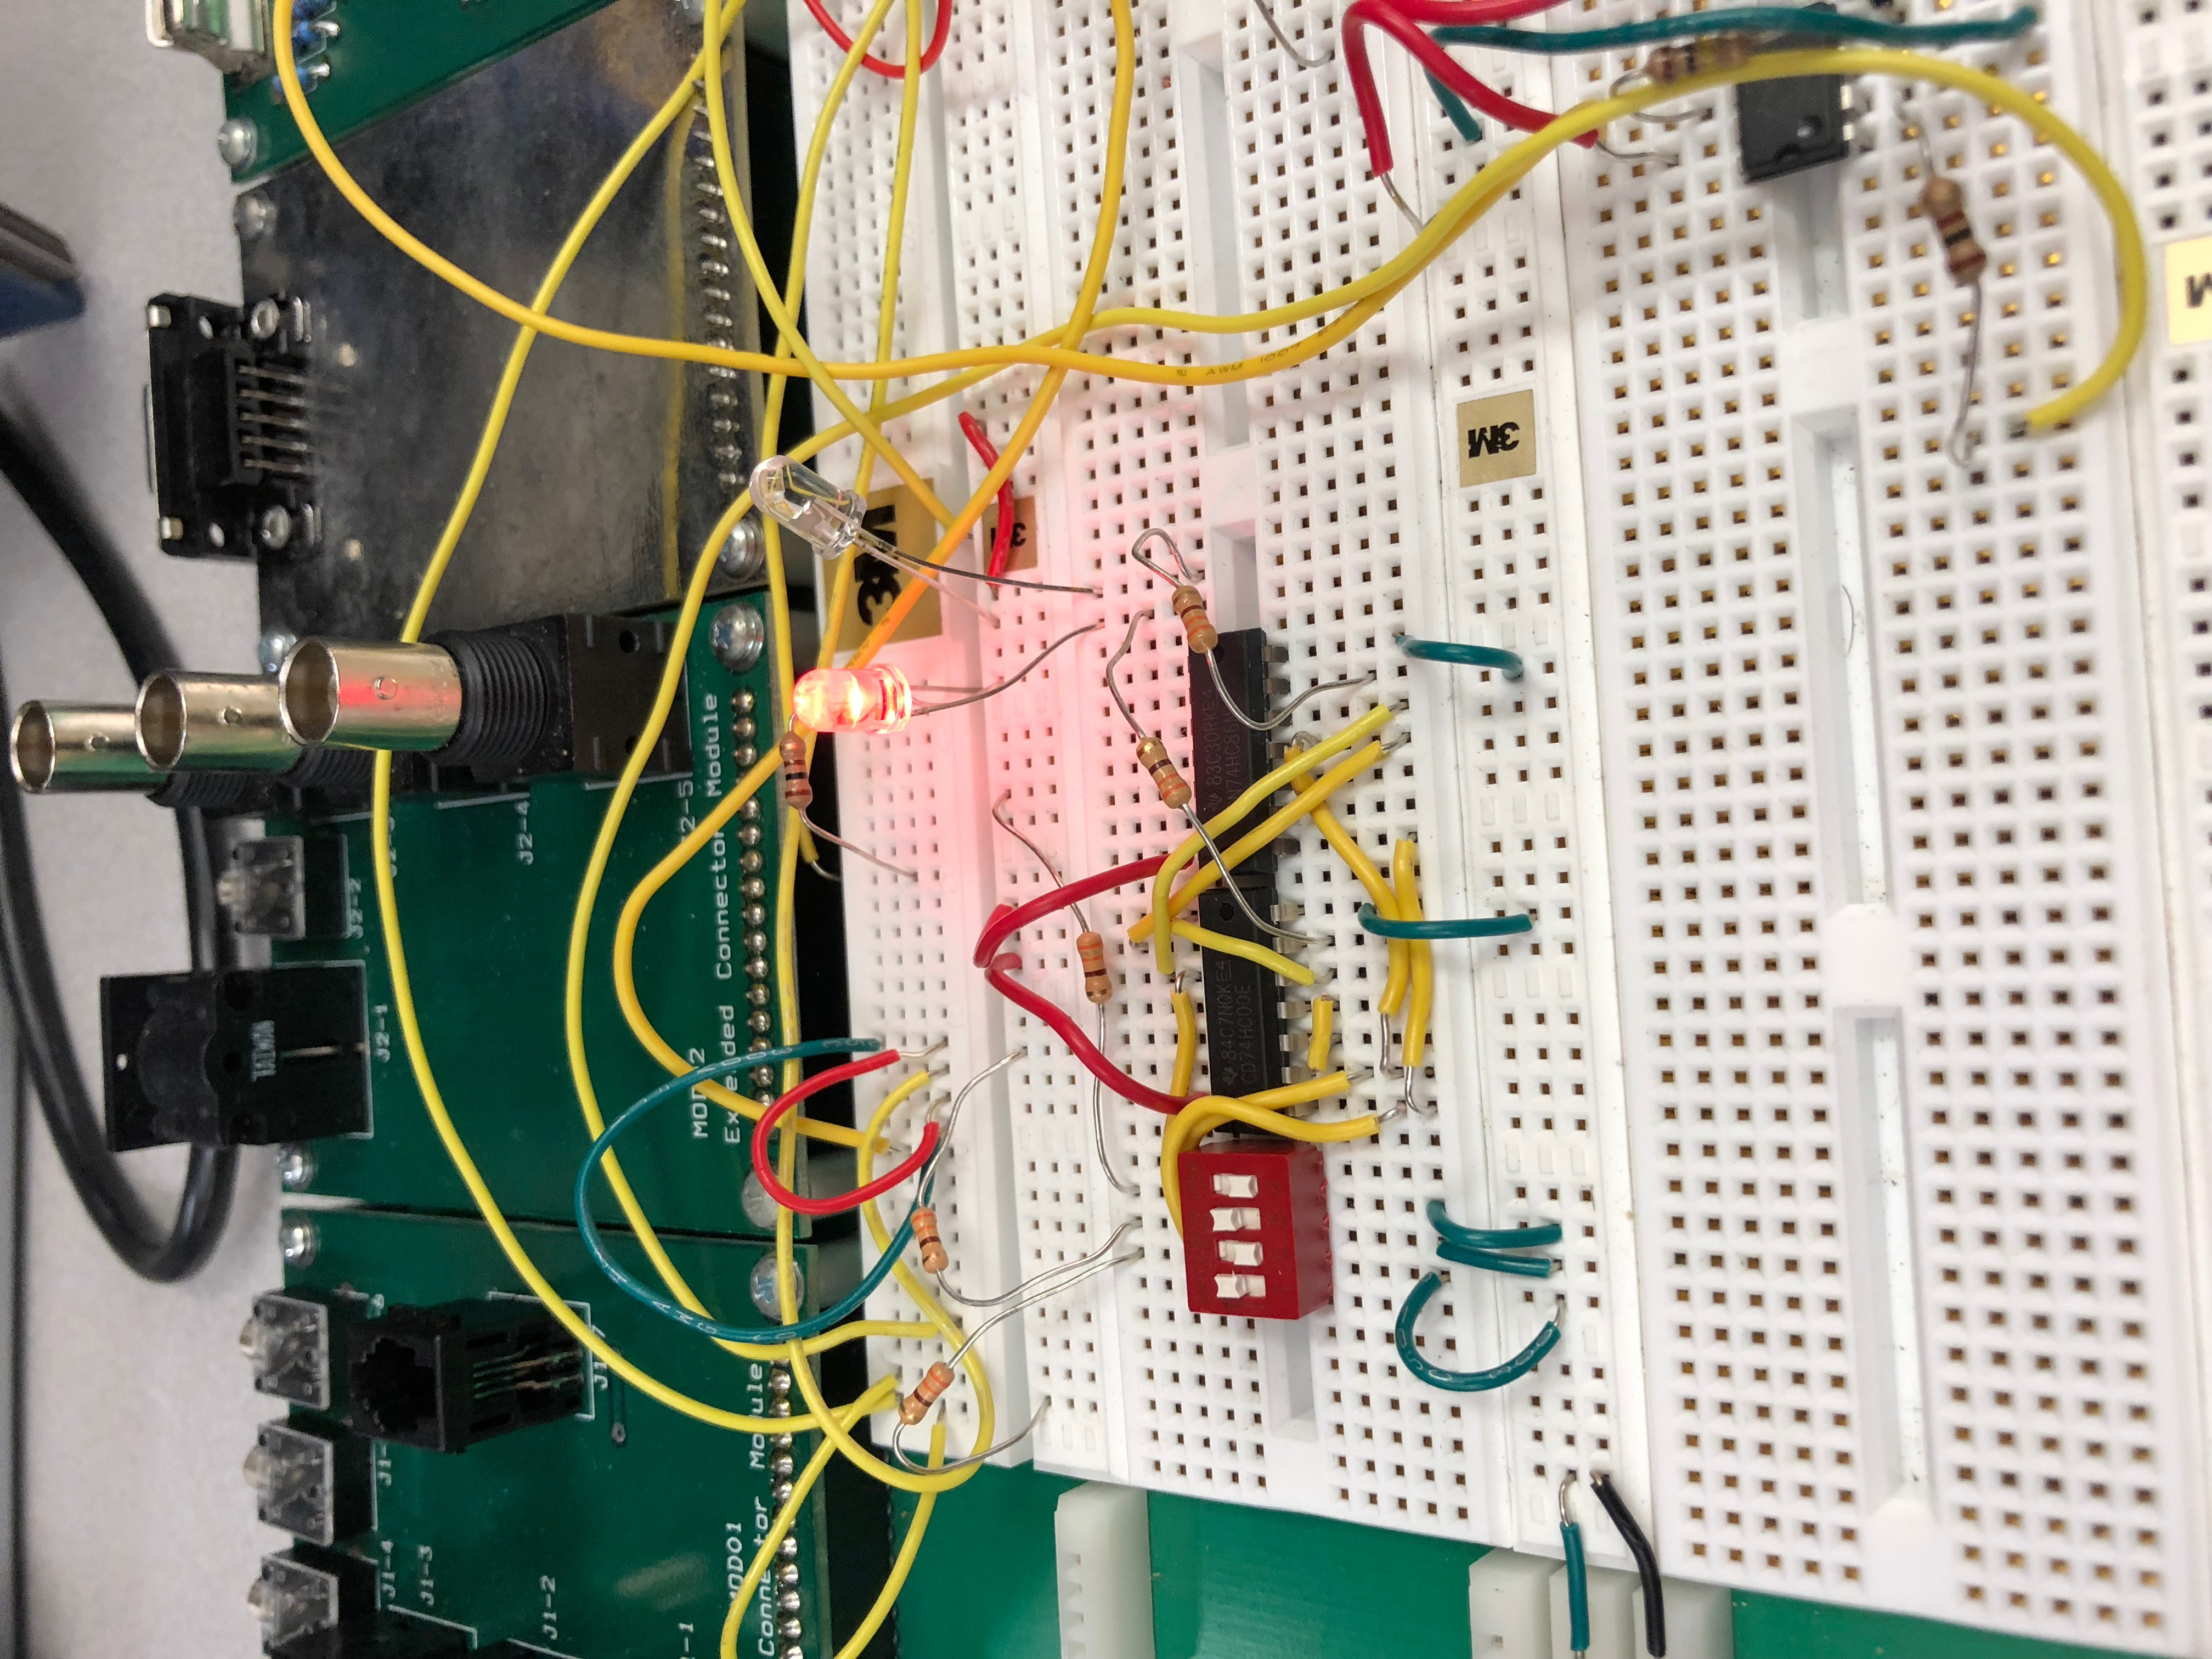
\includegraphics[scale=0.07]{images/101led.jpg}
		\caption{101 Input with 10 Output}
	\end{figure}
\end{centering}

\begin{centering}
	\begin{figure} [H]
		\centering
		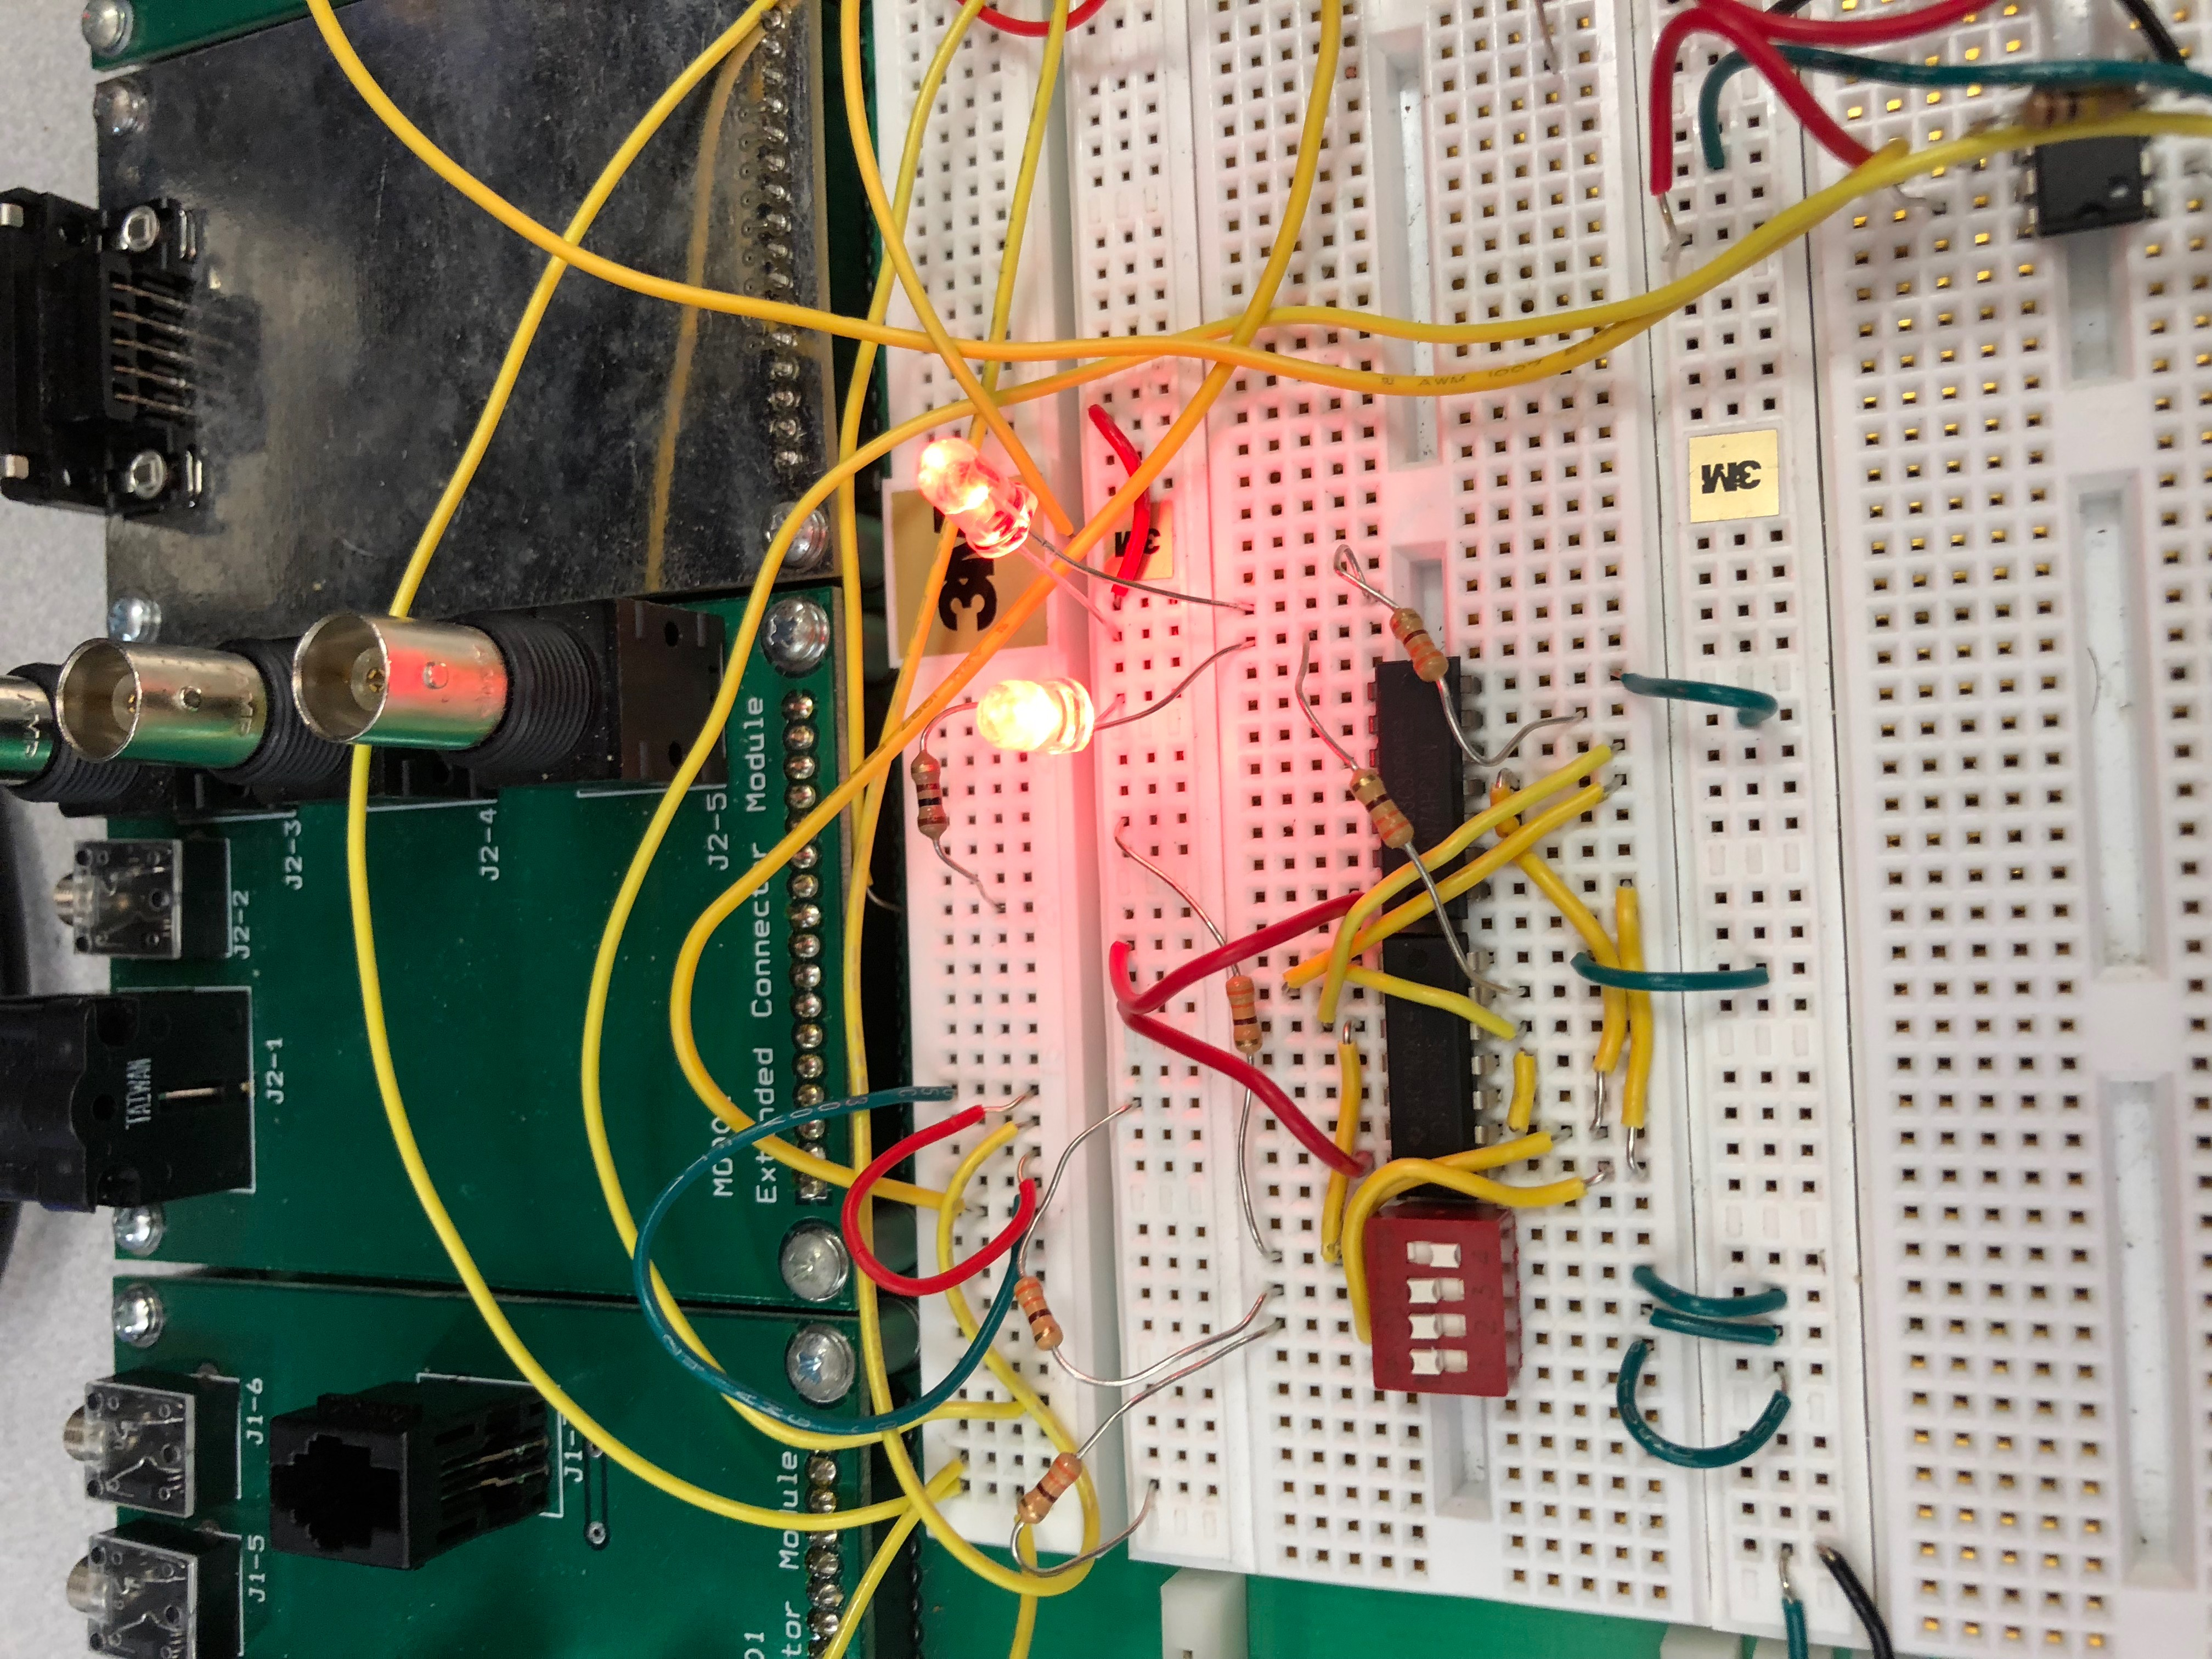
\includegraphics[scale=0.07]{images/111led.jpg}
		\caption{111 Input with 11 Output}
	\end{figure}
\end{centering}

\medskip


\section{References}
https://www.ece.rice.edu/~dpr2/elec240/lab7/experiment\_7-1/

\medskip



\section{Conclusion}

In part A, we learned the various circuit elements and truth tables needed to create a full adder. By adding various truth tables in series, a three bit adder can be created with a carry and sum term. In part B, we combined the truth tables into two that had the desired carry and sum terms. However, this was not done in terms of NAND and XOR, so using DeMorgan's law, these tables were modified to work with only NAND and XOR components. In Part C, we physically created the circuit, and the successful outputs were shown in the Results and Discussion section. Using the given components, the logic checked out, and the full-adder was successful.	

\medskip


\section{Errors}

Since this was a relatively straightforward lab with boolean outputs that returned what was planned, so no errors were experienced. However, if the outputs do not come out as planned possible errors can be attributed to poor wire management or human error.

\medskip


\end{document}
